% ============================================================================
% DHG508 Final Design Paper & Post-Mortem — Motif Atlas
% Lingnan University — Critical Digital History
%
% OVERLEAF SETUP:
%   1. Upload dhg508-overleaf-template.zip (or a zip of this paper/ folder
%      + schematic.png) to Overleaf (New Project -> Upload Project)
%   2. Menu (top left) -> Compiler -> XeLaTeX
%   3. Click Recompile
% ============================================================================

\documentclass[12pt,a4paper]{article}

\usepackage{fontspec}
\newcommand{\MainLatinFont}{Times New Roman}
\newcommand{\FallbackLatinFont}{TeX Gyre Termes}
\newcommand{\MainCJKFont}{Noto Serif CJK SC}
\newcommand{\FallbackCJKFont}{FandolSong-Regular.otf}

\IfFontExistsTF{\MainLatinFont}
  {\setmainfont{\MainLatinFont}}
  {\setmainfont{\FallbackLatinFont}}

\usepackage{xeCJK}
\IfFontExistsTF{\MainCJKFont}
  {\setCJKmainfont{\MainCJKFont}}
  {\IfFontExistsTF{Songti SC}
    {\setCJKmainfont{Songti SC}}
    {\IfFontExistsTF{SimSun}
      {\setCJKmainfont{SimSun}}
      {\setCJKmainfont{\FallbackCJKFont}}}}

\usepackage[a4paper, margin=1in]{geometry}
\usepackage{setspace}
\usepackage{booktabs}
\usepackage{array}
\usepackage{graphicx}
\usepackage{csquotes}

% Chicago Manual of Style 18th ed., Notes-Bibliography (BibLaTeX + Biber)
\usepackage[notes, backend=biber, autolang=other, isbn=false]{biblatex-chicago}
\addbibresource{references.bib}

\renewcommand{\footnotesize}{\fontsize{10}{12}\selectfont}
\usepackage[hidelinks]{hyperref}

\title{\textbf{Motif Atlas: A Comparative Mythology Explorer}\\[0.3em]
\large Design Rationale, Evidence Boundaries, and Post-Mortem}
\author{CHU Man\\Lingnan University $\cdot$ DHG508 Critical Digital History\\
\small Live URL: \url{https://motif-atlas-jwp.pages.dev} $\cdot$ Repo: \url{https://github.com/oliviaaaaa-chu/dhg508-final-project}}
\date{25 November 2026}

\begin{document}
\maketitle

\begin{abstract}
\noindent
The Motif Atlas is a single-page web application for searching, comparing,
mapping and graphing 5{,}494 mythological and religious texts from 39
traditions, and for talking with 153 clearly-labelled fictional characters.
It asks: how can the public be invited into comparative mythology without
smuggling in one ``correct'' classification scheme? The project separates
documented facts (\emph{据}), inferences (\emph{推断}) and design inventions
(\emph{设}) at every layer --- source metadata and sensitivity flags in the
data, a deliberately coarse motif layer whose borrowings from Thompson's
index are named, and a chat whose dramatic voices are banners rather than
authorities. The main takeaway: an interactive medium can \emph{show} the
machinery of interpretation instead of hiding it, and that honesty can be
made testable.
\end{abstract}

\onehalfspacing

\section{Historical Question and Medium}

Comparative mythology has always been an art of classification: Stith
Thompson's \emph{Motif-Index} sorted the world's narratives into numbered
atoms that scholars still cite today.\autocite{thompson1955motif} But as
recent work on machine-readable re-indexings shows, applying that scheme
outside the culture that produced it distorts what it touches: motifs are
context-free atoms that rarely align across traditions, and the indexing
team's own perspective leaks into every tag.\autocite[6]{jokisch2025motif} This raises
the project's historical question: \emph{how can myths and religious texts
from 39 traditions be compared side by side without pretending they fit one
neutral scheme --- and can a tool make its own interpreting visible to its
users?}

A static essay or film can only \emph{describe} such comparison; an
interactive medium can \emph{perform} it, and let the visitor see the seams.
Every view of the Atlas is therefore an exposed interpretive act: Search
explains ``why matched'' for each hit; Compare shows shared motifs and
verbatim quotes between any two texts; Map pins every myth at a coordinate
that is labelled a claim, not a fact; Network graphs similarity with a
threshold slider the user controls; and the Character Chat converses with
fictional figures whose scholarly mode cites corpus passages with a
confidence value. The medium is the argument: instead of hiding
classification behind polished prose, the Atlas shows the classification
step in every view and admits that it is one scheme, not \emph{the} scheme.

\section{Sources and Scholarly Conversation}

The corpus contains 5{,}494 texts across 39 traditions, drawn from
public-domain archives such as Project Gutenberg and the Internet Sacred
Texts Archive.\autocite{gutenberg,sacredtexts} Each text records the
archive, exact work, translator, a working URL and a licence, and carries
1--4 verbatim excerpts (13{,}875 passages, each also rendered in Traditional
Chinese). The mandatory sensitivity flag is enforced by the build script:
a text flagged \texttt{restricted: true} fails validation, so excluded
traditions are kept out by the pipeline rather than by memory. The limits
are real: public-domain sources skew towards older --- often Victorian ---
translations; the collection excludes restricted traditions by design; and
it has honest gaps (the corpus contains no Adam and Eve text at all, which
a playtester caught by searching for the Garden of Eden).

The design responds to four scholarly works, each read in full during Week
9. First, Jokisch's case study of a machine-readable Motif-Index quantifies
the classification problem: in a 1{,}969-narrative South American subset,
roughly 81\% of cross-cultural pairings share only one exact motif, and
``not many things in scholarship are as treacherous as a bad
classification.''\autocite[31]{jokisch2025motif} The Atlas answers with a
deliberately coarse tag layer --- 270 motifs grouped into 28 cross-tradition
families with bilingual descriptions --- which borrows Thompson and ATU codes
where they exist (for searchability) while stating openly that borrowing
preserves search and hides emic meaning. Second, critical cartography's
claim that ``maps make reality as much as they represent
it''\autocite[15]{crampton2005critical} grounds the Map view: its subtitle
says that pins for myth places are interpretive claims, symbolic or
otherworldly places get neutral inland coordinates with explanatory notes,
and the placement questions raised in the research journal (disputed
territories, shared myths, shifting borders) are documented rather than
resolved. Third, Noh and Hong's museum study found that a re-enacted
historical figure was the most engaging condition yet the \emph{worst} at
delivering knowledge, and they recommend an objective ``docent'' voice
wherever objectivity is in
doubt.\autocite[9, 12--13]{noh2021chatbots} The Atlas's chat implements
exactly that split --- a scholarly mode citing only corpus passages with
confidence, and a dramatic mode under a permanent fictionality banner.
Fourth, Zheng et al.\ show across four model families that persona framing
in system prompts does not improve answer
accuracy,\autocite[15126]{zheng2024personas} so the chat's honest claims are
engagement and interpretation, never accuracy --- a limits finding kept
separate from the three historical-argument works.

\section{Architecture and Boundaries}

Data flows one way: curated batches in \texttt{data/raw/} are merged and
validated by \texttt{scripts/01\_build\_corpus.py} into the frozen corpus
\texttt{src/data/texts.json}, which is served as \texttt{public/corpus.json}
and fetched lazily by the app (never blocking first paint). Search combines
a TF-IDF engine with pre-computed 384-dimensional MiniLM embeddings and a
similarity matrix built offline by
\texttt{scripts/04\_semantic\_cache.py}. The UI is Vite + React with
Tailwind, Leaflet for the Map, d3-force for the Network, and Zustand for
state. The Character Chat calls a Cloudflare Pages Function
(\texttt{/api/chat}) that proxies DeepSeek with the key kept server-side,
falling back to a local scripted engine offline. Deployment respects
Cloudflare Pages' 25\,MiB per-file limit: the corpus is split into part
files and the ONNX runtime wasm is pinned from a CDN instead of bundled.

The historical boundaries are explicit. Only public-domain sources are
collected, with licence and URL per text. Restricted traditions stay
excluded --- enforced at validation time, with the chat roster filtered
through the same curatorial policy as the corpus. The chatbot is always
labelled fictional. The corpus is frozen for this cycle (5{,}494 texts), and
\texttt{period} records a text's date of composition or recording, never
``ancient'' alone. Figure~\ref{fig:schematic} shows the resulting
architecture and interaction flow.

\begin{figure}[htbp]
  \centering
  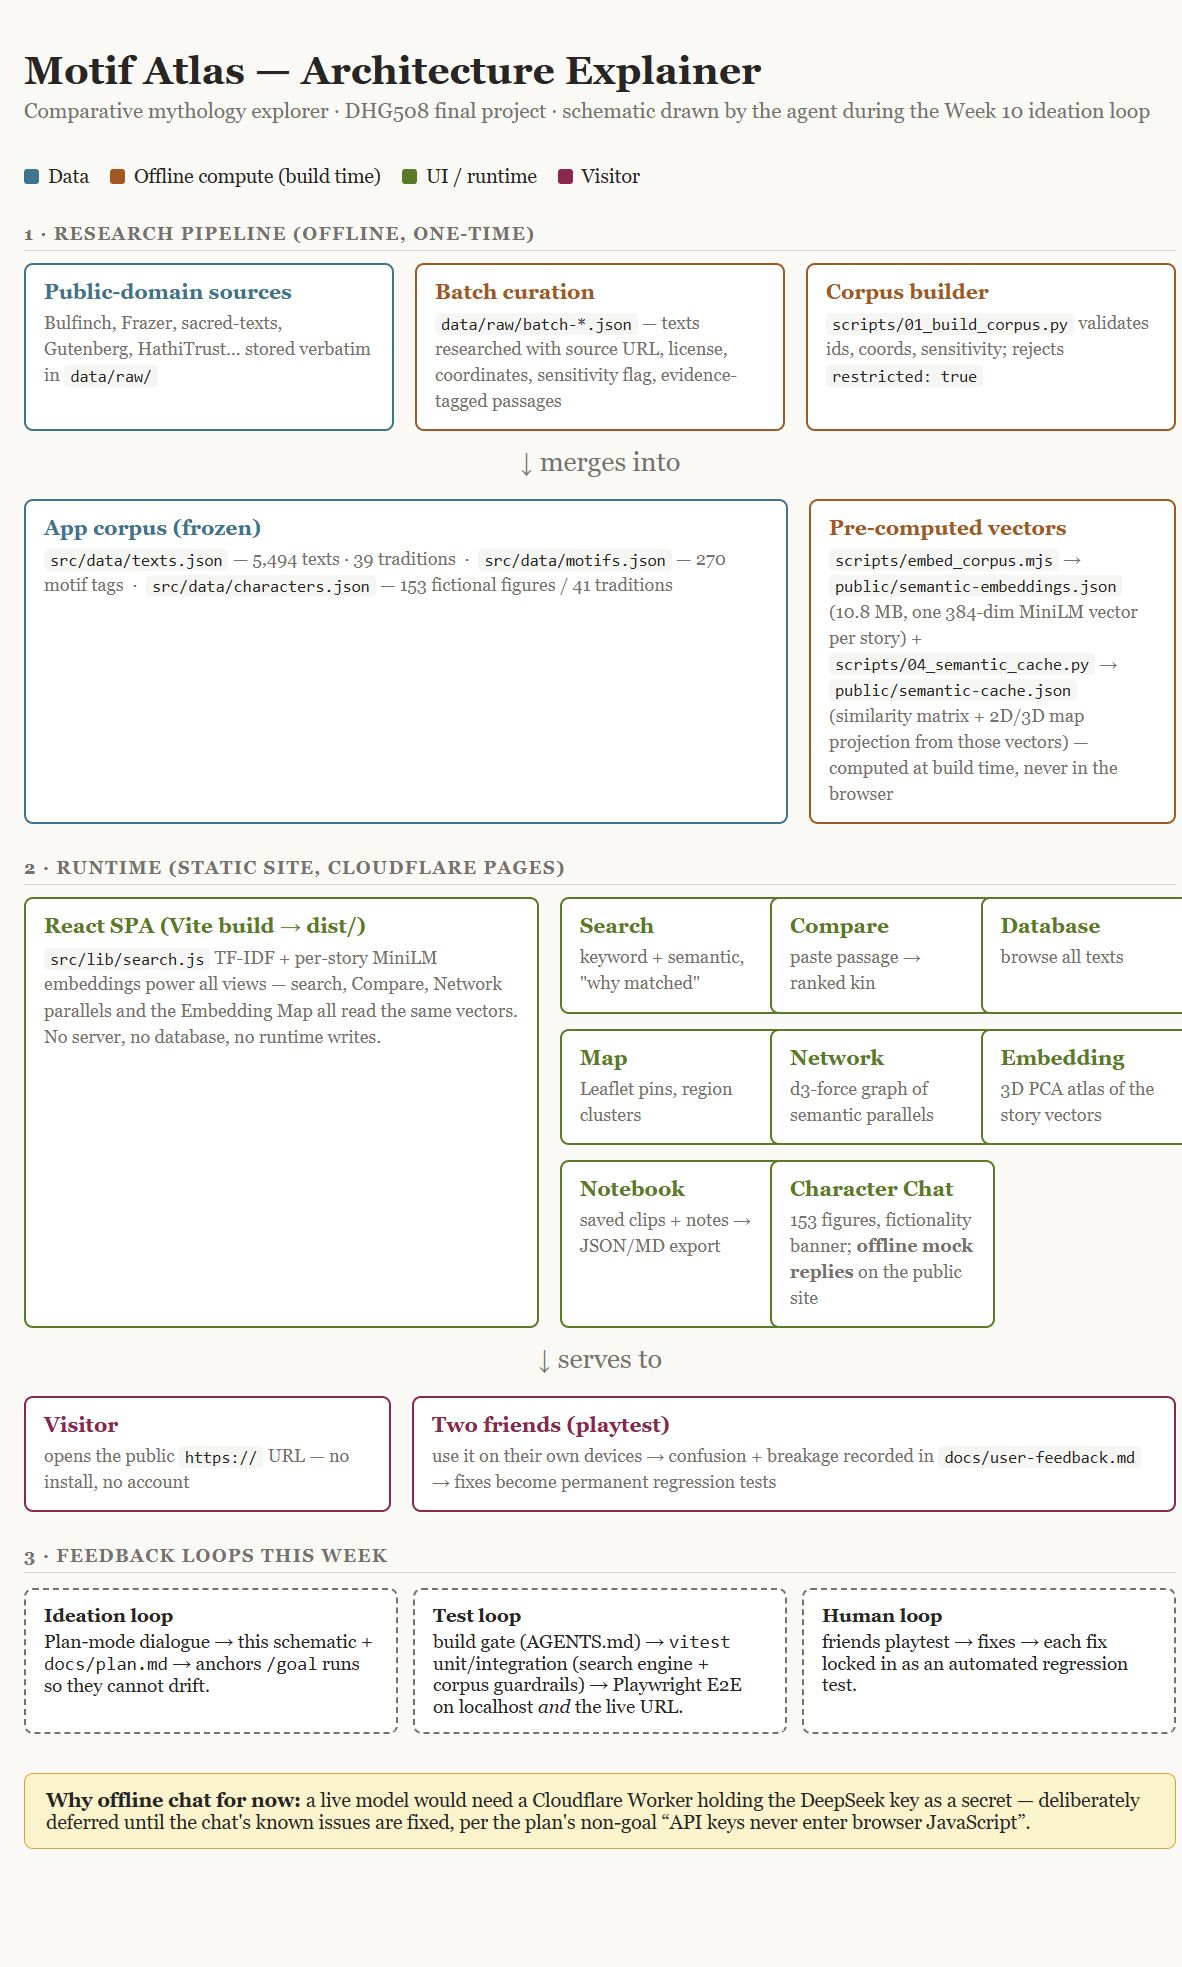
\includegraphics[width=0.92\textwidth]{schematic.png}
  \caption{Project architecture and interaction flow.}
  \label{fig:schematic}
\end{figure}

\section{Evidence Table}

Table~\ref{tab:evidence} is generated from \texttt{evidence.csv} by
\texttt{make\_evidence\_table.py}; rows are never hand-typed into LaTeX.
It records, for each major claim or design element, its evidence, locator,
evidence tier (\emph{据} documented, \emph{推断} inferred, \emph{设}
invented) and its stated limit --- including the two design inventions that
the scholarly findings alone do not justify (the coordinate convention and
the mode split) and the pipeline-enforced corpus rules.

\begin{table}[htbp]
  \centering
  \footnotesize
  \singlespacing
  \renewcommand{\arraystretch}{1.25}
  % Auto-generated from evidence.csv by make_evidence_table.py — edit the CSV, not this file.
\begin{tabular}{p{0.27\textwidth}p{0.20\textwidth}p{0.13\textwidth}p{0.08\textwidth}p{0.22\textwidth}}
  \toprule
  \textbf{Claim / Element} & \textbf{Source / File} & \textbf{Locator} & \textbf{Level} & \textbf{Boundary / Limit} \\
  \midrule
  \textasciitilde{}81\% of cross-cultural narrative pairings share only one exact motif, so context-free motif atoms barely align across traditions & Machine-readable Motif-Index case study on a 1,969-narrative South American subset & Jokisch 2025 pp. 29-31 & 据 & One regional subset; finding applied by analogy and not measured on the Atlas corpus \\
  Motif tagging by a single team exhibits encoder bias, so the tagging scheme itself must be exposed as interpretive & "The entire motif mapping was done by the same team and therefore exhibits encoder bias"; "Not many things in scholarship are as treacherous as a bad classification" & Jokisch 2025 pp. 6 31 & 据 & Writes about their own project; it motivates but does not prove the Atlas's design \\
  The 270-tag motif layer is deliberately coarse (28 cross-tradition families) and borrows Thompson/ATU codes where they exist & src/data/motifs.json records Thompson codes; student journal weighs what borrowing preserves (searchability) against what it hides (emic meaning) & src/data/motifs.json; journal 2026-11-03 axis 1 & 推断 & Code reuse aids search but imports Thompson's Western ordering of motifs \\
  Map pins for myth places are interpretive claims rather than data points & Crampton and Krygier: "maps make reality as much as they represent it"; the Atlas Map subtitle states the same to its users & Crampton and Krygier 2005 p. 15; Map view UI & 据 & The scholarly claim is documented; the subtitle wording is the design's own \\
  Symbolic or otherworldly places receive a neutral inland coordinate plus an explanatory note & Corpus template field rule "note how you chose it" and student placement questions (disputed territories; shared myths; shifting borders) & README corpus fields; journal 2026-11-03 axis 2 & 设 & A design convention; no historical source prescribes a coordinate rule \\
  Re-enacted personas raise engagement and emotional connection but lower knowledge delivery, so an objective voice must remain available & Museum study comparing a re-enacted King chatbot with a docent & Noh and Hong 2021 pp. 9 12-13 & 据 & One museum study in Korea; generalising it to 153 fictional figures is the Atlas's inference \\
  Persona framing does not improve answer accuracy, so the chat's honest claims are engagement and interpretation only & Across 4 LLM families and 162 personas, no statistically significant accuracy gain over control & Zheng et al. 2024 pp. 15126 15134 & 据 & Objective MMLU tasks and open-weight models only; does not measure role-play engagement \\
  Scholarly chat mode cites only real corpus passages with confidence while dramatic mode is banner-labelled fictional & src/lib/mockChat.js mode split; plan red line "the chatbot is always labelled fictional" & src/lib/mockChat.js; docs/plan.md section 3 & 设 & The split is a design invention responding to the two documented findings above; citations are only as good as the public-domain corpus \\
  Traditions where myth and religion share one origin receive a myth-religion category instead of a forced split & category field documentation naming Hindu / Norse / Yoruba / Afro-Atlantic / Celtic & README category field & 推断 & Interpretive division; reasoning is noted in the data where ambiguous \\
  Search bridges singular and plural stems and Greek/Roman name equivalences so queries find the same stories & Playtest found "apple/appl" split and Hercules vs Heracles misses; stemmer fixed and name-equivalence table added, each with regression tests & docs/user-feedback.md item 4; tests/engine.test.js & 据 & The equivalence table covers common pairs only \\
  The chat roster passes the same curatorial policy as the corpus, so restricted traditions stay excluded everywhere & Six figures from excluded traditions leaked into the picker; roster now policy-filtered with a unit test & docs/user-feedback.md item 2; tests/corpus.test.js & 据 & The exclusion policy itself is the design's own curatorial decision \\
  Corpus frozen at 5494 texts / 39 traditions / 270 motifs with source URL / license / mandatory sensitivity flag per text; restricted traditions fail validation & docs/plan.md scope and boundaries plus scripts/01\_build\_corpus.py validation & docs/plan.md; scripts/01\_build\_corpus.py & 据 & Public-domain translations only; corpus gaps are logged in questions.md (e.g. no Adam and Eve text) \\
  \bottomrule
\end{tabular}

  \caption{Claims and design elements with locators, evidence tiers
  (\emph{据} documented, \emph{推断} inferred, \emph{设} invented), and limits.}
  \label{tab:evidence}
\end{table}

\section{Verification and Playtesting}

Thirty-one unit and integration tests (Vitest) act as historical guardrails:
they verify corpus integrity (required fields, coordinates, sensitivity
flags, exclusion of restricted traditions), the search engine (stemming,
name-equivalence resolution, chat policy), and the offline chat fallback.
Nine Playwright end-to-end tests run against the production build and
against the live URL, and the suite fails on any console or page error.

Two external users then played the live site on 18 November 2026. Tester~A,
on a phone in Canada, reported that the site would not open at all: the
diagnosis was a 23.4\,MB JavaScript bundle (the whole corpus compiled into
it) plus a blocking top-level \texttt{await}; the fix moved the corpus to a
lazily-fetched file with a visible loading screen and shrank the bundle to
1.19\,MB, locked in by an E2E test that fails if first load exceeds 3\,MB of
script. Tester~A then filed five further reports, each producing a fix and
a regression test: an explicit ``open details'' button for database cards;
the chat picker leaking six figures from traditions the curatorial policy
excludes (the roster is now policy-filtered, with a unit test); mislabelled
``Philippines'' and ``Maya'' entries; three search bugs (a stemmer that
split ``apple'' and ``apples'' onto different index terms, matched-terms
display showing raw stems, and ``Hercules''/``Heracles'' resolving to
different stories --- the corpus simply had no Adam and Eve text, which was
logged as a corpus gap rather than disguised as a bug); and a Network view
that froze the page by synchronously simulating all ${\sim}5{,}400$ nodes
for 420 ticks on every threshold change (now only edge-connected nodes
simulated, edges capped at 500, layout settles after 120 ticks, slider
deferred). Tester~B's report requested a Traditional Chinese interface; the
bilingual dictionaries were re-enabled, 24 untranslated strings were
translated, and an E2E test asserts the choice persists across reload.

\section{Post-Mortem}

\begin{enumerate}
  \item \textbf{What worked:} Turning every historical rule into a test the
  moment it was decided --- validation-time exclusion of restricted
  traditions, the sensitivity flag, the fictionality red line --- meant the
  guardrails accumulated into the project's real specification. The
  corpus-build pipeline (edit batches, re-run the script) made a 5{,}494-text
  corpus maintainable by one person. Generating this paper's evidence table
  from CSV rather than typing LaTeX rows kept the claim/limit record honest.
  The scholarly-search route (OpenAlex, verified publisher PDFs, quotes with
  locators in the research journal) made Section~2 citable rather than
  decorative.
  \item \textbf{What failed:} The first deployment carried a 23.4\,MB bundle
  and a blocking top-level \texttt{await} that made the site unusable on
  phones; the Network view froze on real corpus sizes; the stemmer ranked
  singular and plural queries differently; six excluded-tradition figures
  reached the chat picker. Each failure was found by a user or a test, and
  each ended as a permanent regression test.
  \item \textbf{What changed:} The app grew from a 207-text Week~9 demo to
  5{,}494 texts across 39 traditions, which forced an architecture inversion
  (corpus out of the bundle, lazy hydration, CDN-pinned wasm). The bilingual
  corpus --- 13{,}875 Traditional Chinese passages, batch-translated then
  agent-translated --- was added only after Tester~B asked for it, and the
  chat roster was placed under the same curatorial policy as the corpus
  after the picker leak.
  \item \textbf{Limits and AI tools:} Semantic matching (TF-IDF plus MiniLM
  embeddings) remains coarse; Jokisch's 81\% finding means cross-tradition
  motif alignment is interpretive no matter how the engine is tuned. The
  corpus inherits the age and bias of public-domain translations, and gaps
  (no Eden text) are logged rather than filled. The persona chat is bounded
  by context windows and by the policy that dramatic mode must never pose as
  scholarship. AI tools used: OpenCode coding agents for build, tests,
  deployment and this paper's scaffolding; DeepSeek for the chat proxy and
  batch translation; a MiniLM model from Hugging Face for embeddings; every
  AI output was curated, labelled, and remains reviewable in the repository.
\end{enumerate}

\singlespacing
\printbibliography[title={Bibliography}]

\end{document}
